\section{Results \& Discussion}
\subsection{X-ray reflectometry}
The chemically-consistent model was co-refined across XRR measurements at all four surface pressures for each phospholipid.
The resulting XRR profiles and associated SLD profiles are shown in Figure~\ref{fig:xrrref}.
Table~\ref{tab:xrrref3} gives the parameters for each of the phospholipids at the second highest surface pressure measured, as well as the details of $\phi_h$, as determined from Equation~\ref{equ:phih}.\footnote{The parameters at the other surface pressures may be found in Appendix~\ref{refl1app}.}
%
\begin{figure}
    \centering
    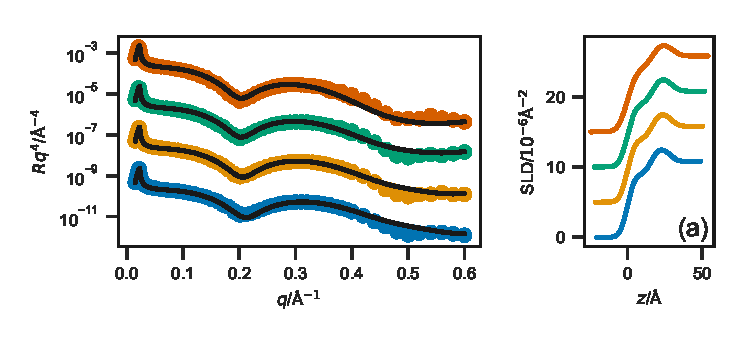
\includegraphics[width=\textwidth]{reflectometry1/dppc_xray_ref_sld}
    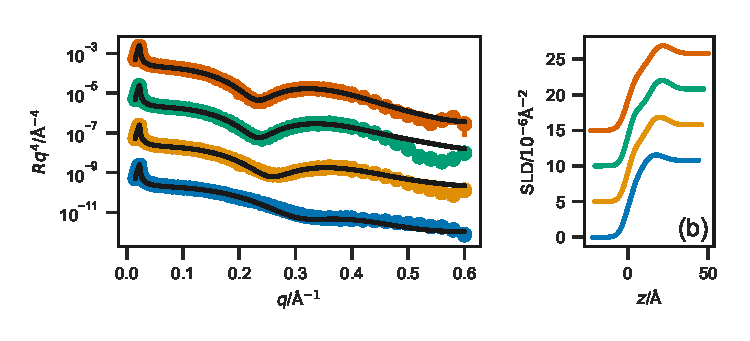
\includegraphics[width=\textwidth]{reflectometry1/dmpc_xray_ref_sld}
    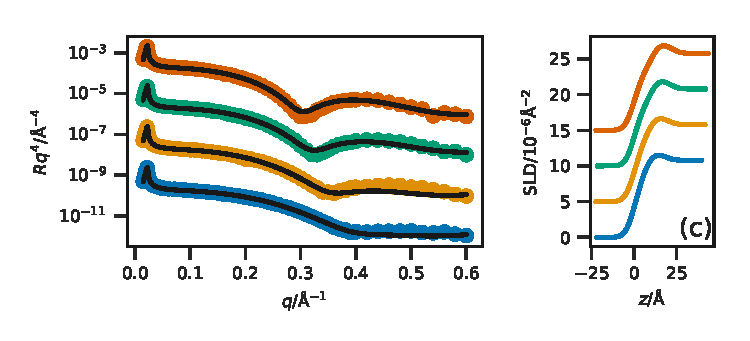
\includegraphics[width=\textwidth]{reflectometry1/dlpc_xray_ref_sld}
    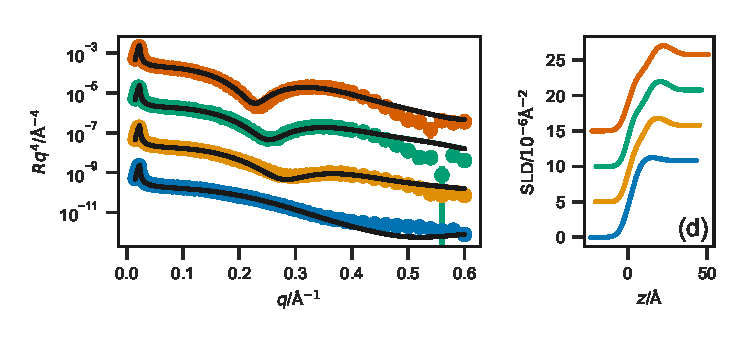
\includegraphics[width=\textwidth]{reflectometry1/dmpg_xray_ref_sld}
    \caption{The XRR profiles (left) and SLD profiles (right) for each of the four phospholipids; (a) DPPC, (b) DMPC, (c) DLPC, and (d) DMPG, at the four measured surface pressures; increasing in surface pressure from blue, orange, green to red. The different surface pressure XRR profiles have been offset in the \emph{y}-axis by two orders of magnitude and the SLD profiles offset in the \emph{y}-axis by \SI{5e-6}{\per\angstrom\squared}, for clarity.}
    \label{fig:xrrref}
\end{figure}
%
%
\begin{table}
    \centering
    \small
    \caption{The best-fit values, and associated \SI{95}{\percent} confidence intervals for each of the varying parameters for each phospholipid at the second highest surface pressure measured from XRR. The values of $\phi_h$ were obtained from the appropriate use of Equation~\protect\ref{equ:phih}. Surface pressure has been abbreviated to SP.}
    \label{tab:xrrref3}
    \begin{tabular}{l | l l l l}
        \toprule
        Phospholipid & DPPC & DMPC & DLPC & DMPG \\
        SP/\si{\milli\newton\per\meter} & 25 & 30 & 30 & 25 \\
        \midrule
        $V_t$/\si{\angstrom\cubed} & \input{output/reflectometry1/dppc_xray/dppc_xray-V_t} & \input{output/reflectometry1/dmpc_xray/dmpc_xray-V_t} & \input{output/reflectometry1/dlpc_xray/dlpc_xray-V_t} & \input{output/reflectometry1/dmpg_xray/dmpg_xray-V_t} \\
        $V_h$/\si{\angstrom\cubed} & \input{output/reflectometry1/dppc_xray/dppc_xray-V_h} & \input{output/reflectometry1/dmpc_xray/dmpc_xray-V_h} & \input{output/reflectometry1/dlpc_xray/dlpc_xray-V_h} & \input{output/reflectometry1/dmpg_xray/dmpg_xray-V_h} \\
        $d_h$/\si{\angstrom} & \input{output/reflectometry1/dppc_xray/dppc_xray-d_h} & \input{output/reflectometry1/dmpc_xray/dmpc_xray-d_h} & \input{output/reflectometry1/dlpc_xray/dlpc_xray-d_h} & \input{output/reflectometry1/dmpg_xray/dmpg_xray-d_h} \\
        \midrule
        $d_t$\si{\angstrom} & \input{output/reflectometry1/dppc_xray/dppc_xray-d_t_25} & \input{output/reflectometry1/dmpc_xray/dmpc_xray-d_t_30} & \input{output/reflectometry1/dlpc_xray/dlpc_xray-d_t_30} & \input{output/reflectometry1/dmpg_xray/dmpg_xray-d_t_25} \\
        $\sigma_{t,h,s}$/\si{\angstrom} & \input{output/reflectometry1/dppc_xray/dppc_xray_rough_25} & \input{output/reflectometry1/dmpc_xray/dmpc_xray_rough_30} & \input{output/reflectometry1/dlpc_xray/dlpc_xray_rough_30} & \input{output/reflectometry1/dmpg_xray/dmpg_xray_rough_25} \\
        \midrule
        $\phi_h$/$\times 10^{-2}$ & \input{output/reflectometry1/dppc_xray/dppc_xray-phih_25} & \input{output/reflectometry1/dmpc_xray/dmpc_xray-phih_30} & \input{output/reflectometry1/dlpc_xray/dlpc_xray-phih_30} & \input{output/reflectometry1/dmpg_xray/dmpg_xray-phih_25} \\
        \bottomrule
    \end{tabular}
\end{table}
%

Following the structural determination of the monolayer from the XRR measurements.
NR was used to confirm the values of the head and tail group volumes that had been determined.
The resulting NR profiles and associated SLD profiles, at both surface pressures measured can be found in Figure~\ref{fig:nrref}.
Table~\ref{tab:nrref} gives the parameters as determined from the NR measurements, along with $\phi_h$ as determined from Equation~\ref{equ:phih}.
%
\begin{figure}
    \centering
    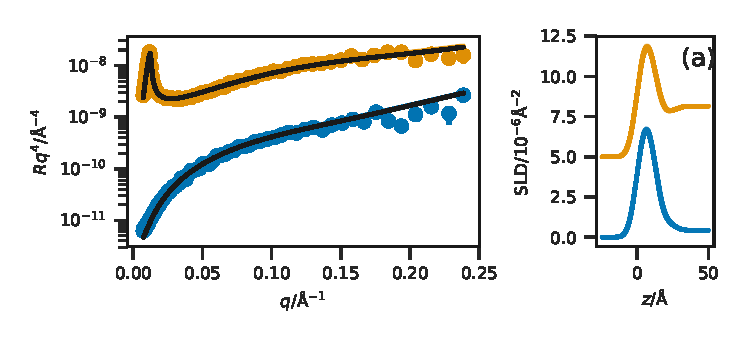
\includegraphics[width=\textwidth]{reflectometry1/dppc_neutron_15_ref_sld}
    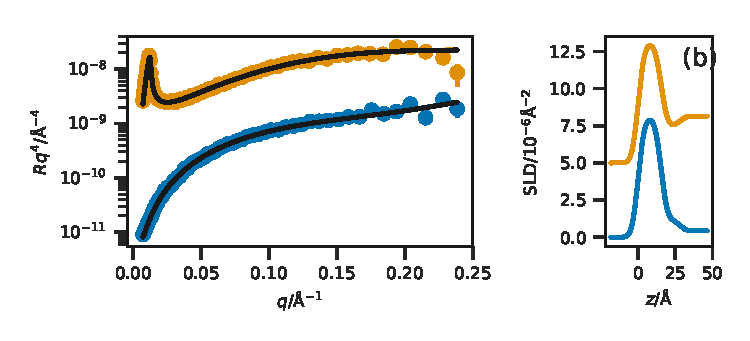
\includegraphics[width=\textwidth]{reflectometry1/dppc_neutron_20_ref_sld}
    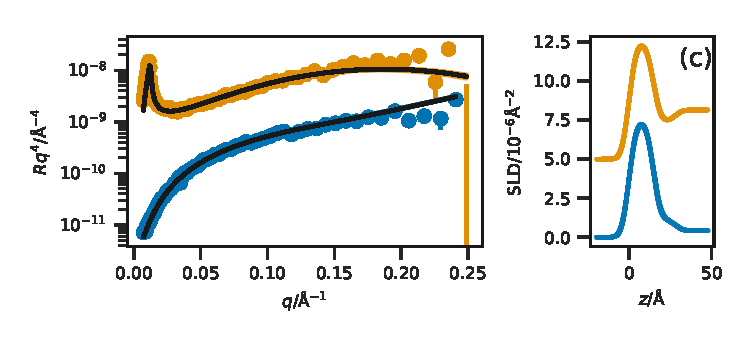
\includegraphics[width=\textwidth]{reflectometry1/dmpc_neutron_20_ref_sld}
    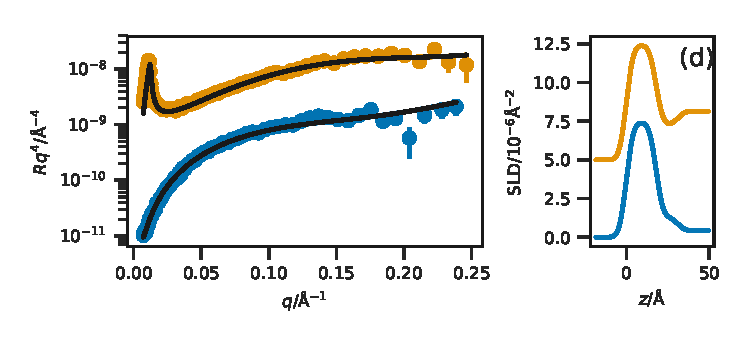
\includegraphics[width=\textwidth]{reflectometry1/dmpc_neutron_25_ref_sld}
    \caption{The NR profiles (left) and SLD profiles (right) for each of the four phospholipids; (a) DPPC at \SI{15}{\milli\newton\per\meter}, (b) DPPC at \SI{20}{\milli\newton\per\meter}, (c) DMPC at \SI{20}{\milli\newton\per\meter}, and (d) DMPC at \SI{25}{\milli\newton\per\meter}, where the blue data indicates the h-DES contrast, while the orange is the hd-DES. The different surface pressure XRR profiles have been offset in the \emph{y}-axis by an order of magnitude and the SLD profiles offset in the \emph{y}-axis by \SI{5e-6}{\per\angstrom\squared}, for clarity.}
    \label{fig:nrref}
\end{figure}
%
%
\begin{table}
    \centering
    \small
    \caption{The best-fit values, and associated \SI{95}{\percent} confidence intervals for each of the varying parameters for each phospholipid at the each surface pressure from NR. The values of $\phi_h$ were obtained from the appropriate use of Equation~\protect\ref{equ:phih}.}
    \label{tab:nrref}
    \begin{tabular}{l | l l l l}
        \toprule
        Phospholipid & DPPC & DPPC & DMPC & DMPC \\
        SP/\si{\milli\newton\per\meter} & 15 & 20 & 20 & 25 \\
        \midrule
        $d_t$\si{\angstrom} & \input{output/reflectometry1/dppc_neutron/dppc_neutron_15-d_t_15} & \input{output/reflectometry1/dppc_neutron/dppc_neutron_20-d_t_20} & \input{output/reflectometry1/dmpc_neutron/dmpc_neutron_20-d_t_20} & \input{output/reflectometry1/dmpc_neutron/dmpc_neutron_25-d_t_25} \\
        $\sigma_{t,h,s}$/\si{\angstrom} & \input{output/reflectometry1/dppc_neutron/dppc_neutron_15_rough_15} & \input{output/reflectometry1/dppc_neutron/dppc_neutron_20_rough_20} & \input{output/reflectometry1/dmpc_neutron/dmpc_neutron_20_rough_20} & \input{output/reflectometry1/dmpc_neutron/dmpc_neutron_25_rough_25} \\
        \midrule
        $\phi_h$/$\times 10^{-2}$ & \input{output/reflectometry1/dppc_neutron/dppc_neutron_15-phih_15} & \input{output/reflectometry1/dppc_neutron/dppc_neutron_20-phih_20} & \input{output/reflectometry1/dmpc_neutron/dmpc_neutron_20-phih_20} & \input{output/reflectometry1/dmpc_neutron/dmpc_neutron_25-phih_25} \\
        \bottomrule
    \end{tabular}
\end{table}
%

\subsection{Effect of compression on the monolayer thickness}
From Tables~\ref{tab:xrrref1}, \ref{tab:xrrref2}, \ref{tab:xrrref3}, \ref{tab:xrrref4}, and \ref{tab:nrref}, it can be seen that, as expected and shown in previous work at the air-water interface,\autocite{mohwald_phospholipid_1990,vaknin_structural_1991} the thickness of the tail layer increases as the number of carbon atoms in the tail chain increases.
Furthermore, the thickness of the tail layers determined here agrees well with values found for water-analogues; \input{output/reflectometry1/dmpc_xray/dmpc_xray-d_t_30}\si{\angstrom} at \SI{30}{\milli\newton\per\meter} in DES compared with \SI{15.8}{\angstrom} at \SI{30}{\milli\newton\per\meter} in water for DMPC, and \input{output/reflectometry1/dppc_xray/dppc_xray-d_t_30}\si{\angstrom} at \SI{30}{\milli\newton\per\meter} in DES compared with \SI{16.7}{\angstrom} at \SI{40}{\milli\newton\per\meter} in water for DPPC.

The variation of the tail layer thickness in the models with surface pressure is given for each phospholipid in Figure~\ref{fig:dtphi}.
For all of the phospholipids, as the surface pressure increases, the thickness of the tail layer also increases to a point before plateauing; for DPPC this occurs at \SI{20}{\milli\newton\per\meter}, DMPC at \SI{30}{\milli\newton\per\meter}, and for DMPG and DLPC can be assumed to be at higher pressures than those studied.
This relationship of increasing tail layer thickness with increasing surface pressure has been noted previously for DMPC\autocite{bayerl_specular_1990} and DPPC\autocite{campbell_structure_2018} at the air-water interface.
This can be easily understood as the angle of the tail group with respect to the surface normal decreasing as the surface pressure increases.
%
\begin{figure}
    \centering
    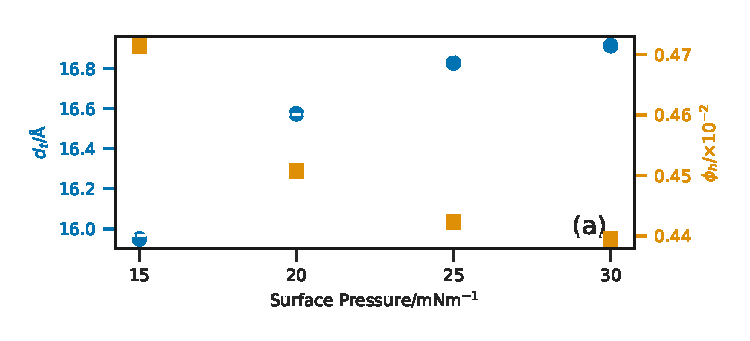
\includegraphics[width=\textwidth]{reflectometry1/dppc_xray_dt_phi}
    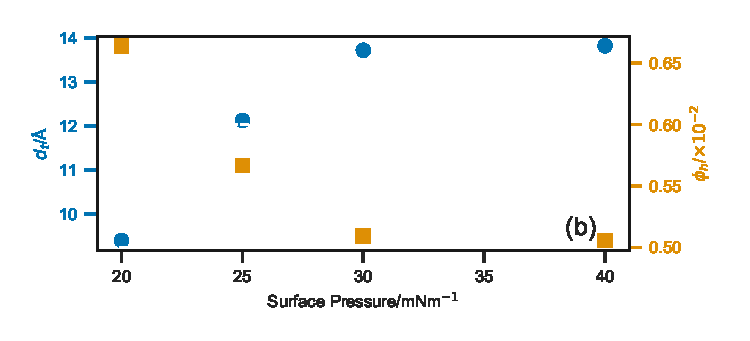
\includegraphics[width=\textwidth]{reflectometry1/dmpc_xray_dt_phi}
    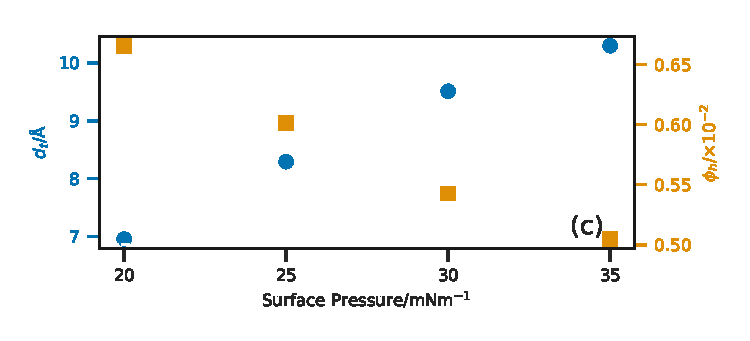
\includegraphics[width=\textwidth]{reflectometry1/dlpc_xray_dt_phi}
    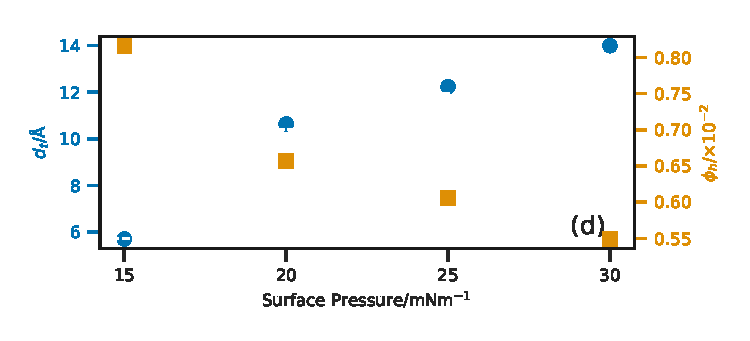
\includegraphics[width=\textwidth]{reflectometry1/dmpg_xray_dt_phi}
    \caption{The variation of tail layer thickness, $d_t$, (blue circles) and head group solvation, $\phi_h$, (orange squares) with surface pressures for each of the four phospholipids; (a) DPPC, (b) DMPC, (c) DLPC, and (d) DMPG.}
    \label{fig:dtphi}
\end{figure}
%

\subsection{Effect of compressure on solvent fraction}
In Figure~\ref{fig:dtphi}, it is clear that for all four phospholipids, as the surface pressure is increased there is a corresponding reduction in the volume fraction of solvent in the phospholipid head layer,
This can be rationalised by considering that when the surface pressure is increased, there is a corresponding increase in surface concentration, hence the free volume available to the solvent is less.
A similar effect has been observed when increasing the surface pressure from \SI{11}{\milli\newton\per\meter} to \SI{31}{\milli\newton\per\meter} for a mixed DMPC/DMPG monolayer at the air-water interface.\autocite{bayerl_specular_1990}

\subsection{Effect of compression on the phospholipid tail component volumes}
It can be seen from comparing Table~\ref{tab:water} with Tables~\ref{tab:xrrref1}, \ref{tab:xrrref2}, \ref{tab:xrrref3}, and \ref{tab:xrrref4} that the volumes of the phospholipid tails are substantially lower in the current measurement than found previously, by other techniques.
It is unlikely that this is a result of the DES subphase, due to the solvophobic nature of these tail groups.
However, a similar reduction has been shown previously,\autocite{campbell_structure_2018} where it was rationalised by the compaction of the monolayer at elevated surface pressure.
In that work, the optimal value for the tail group volume of DPPC was found to be \SI{772}{\angstrom\cubed} at a surface pressure of \SI{35}{\milli\newton\per\meter}, which agrees well with the value of \input{output/reflectometry1/dppc_xray/dppc_xray-V_t.tex}\si{\angstrom\cubed} found in this work at surface pressures of \SIlist{15;20;25;30}{\milli\newton\per\meter}.
The reduction in tail volume was found to be between \SIrange{8}{12}{\percent} for DPPC, DMPC, DLPC when compared with the literature sources at \SIlist{24;30}{\celsius}.
This is close to the maximum compression of \SI{15}{\percent} noted by Small.\autocite{small_lateral_1984}
DMPG shows a small increase in the tail volume when compared with the literature value, albeit at a higher temperature.
However, this value agrees well with that found for DMPC which shares the same tail structure.

\subsection{Solvent effect on the phospholipid head group volume}
Tables~\ref{tab:xrrref1}, \ref{tab:xrrref2}, \ref{tab:xrrref3}, and \ref{tab:xrrref4} give the best-fit values for the head group volumes for each of phospholipids investigated.
Ths three phospholipids with the PC head group are consistent, giving values of \SI{\sim 330}{\angstrom\cubed}, regardless of the tail group.
This agrees well with the values found for the same head component in water, shown in Table~\ref{tab:water}.
Interestingly, the head group volume determined for the PG containing phospholipid is similar to that for the PC head group, with a value of \input{output/reflectometry1/dmpg_xray/dmpg_xray-V_h.tex}~\si{\angstrom\cubed}.
The PG head group volume in water from either DMPG using differential vibrating tube densimetry\autocite{pan_molecular_2012} or POPG using molecular dynamics simulations,\autocite{kucerka_scattering_2012} is noticeably smaller.
This indicates that there may be some effect arising from the solvation of the PG component in the choline chloride:glycerol DES.
However, this has only been shown for a single PG-lipid at the air-DES interface.

The major difference between the two head groups of the phospholipid is that the PG is present as a sodium salt, whereas the PC is zwitterionic.
When in solution the anionic PG head is expected to associate with cations in solution, as it does in water\autocite{grigoriev_effect_1999} where such interactions depend on a variey of factors including the ionic strength.
In the case of a DES, the environment is inherently ionic and therefore the interaction of an anionic phospholipid head may be more complex.
As well as interacting with this sodium, the head is likely to interact with the choline cations, similar to behaviour reported previously for surfactact micelles.\autocite{sanchez-fernandez_counterion_2018}
The extent of interaction with each of the cations is unclear, but regardless it seems likely that the solvation of the PG head is improved in the DES relative to water.
This better solvation would explain the apparent increase in the volume of the PG head since it would result in a swelling of this group through its strong interactions with the solvent.
In the case of PC, the proximity of a local cation within the molecule results in the same folding of the head group seen in water because this interaction is less transient that the equivalent interactions with the solvent.

\subsection{Analysis of neutron reflectometry}
The ability to fit NR data in Figure~\ref{fig:nrref} indicated that the values found for the head and tail groups are consistent between the pair of measurements for the same systems.
It is clear that again stable monolayers of the phospholipids are forming at the air-DES interface and that the volumes determined by XRR measurements are robust enough to be used in the modelling of NR data.
Furthermore, as shown in Table~\ref{tab:nrref}, the trends observed with increasing surface pressure in the XRR models, pertaining to a responsive increase in tail thickness and a decrease in solvent concentration in the head layer are consistent with that found with the NR analysis.

\subsection{Utility of Markov chain Monte Carlo sampling}
The use of MCMC sampling enabled the inverse uncertainties for each of the fitted parameters to be determined as a confidence interval from the PDFs.
The PDFs for DLPC are shown in Figure~\ref{fig:dlpcpdfs}.\footnote{Those for the other phospholipid-XRR and NR measurements can be found in Appendix~\ref{refl1app}.}
These confidence intervals are useful for understanding the probability of the given value, however as discussed in Section~\ref{refl1:anal} these intervals only represent the uncertainty in the experimental data and do not account for systematic uncertainty present in the measurement method.
%
\begin{figure}
    \centering
    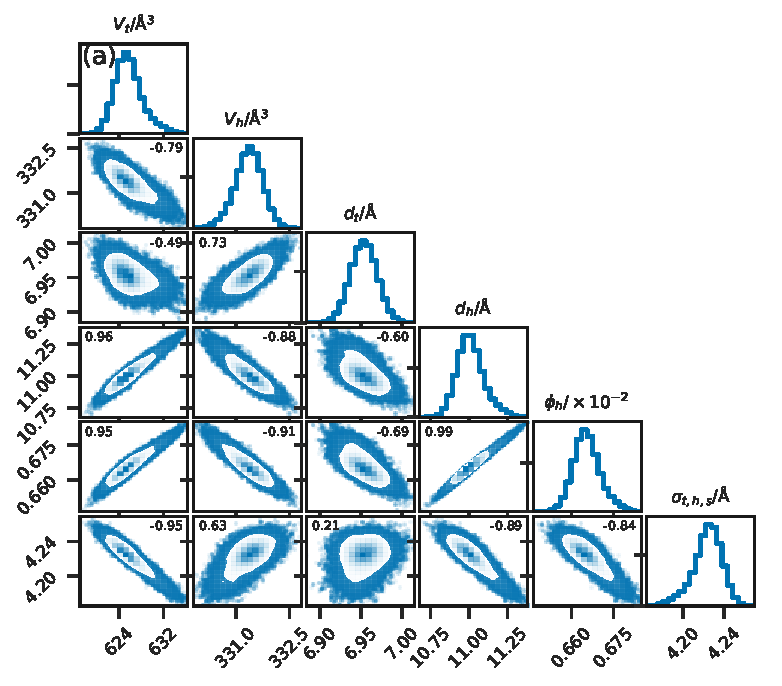
\includegraphics[width=0.49\textwidth]{reflectometry1/dlpc_xray_sp_20_pdf}
    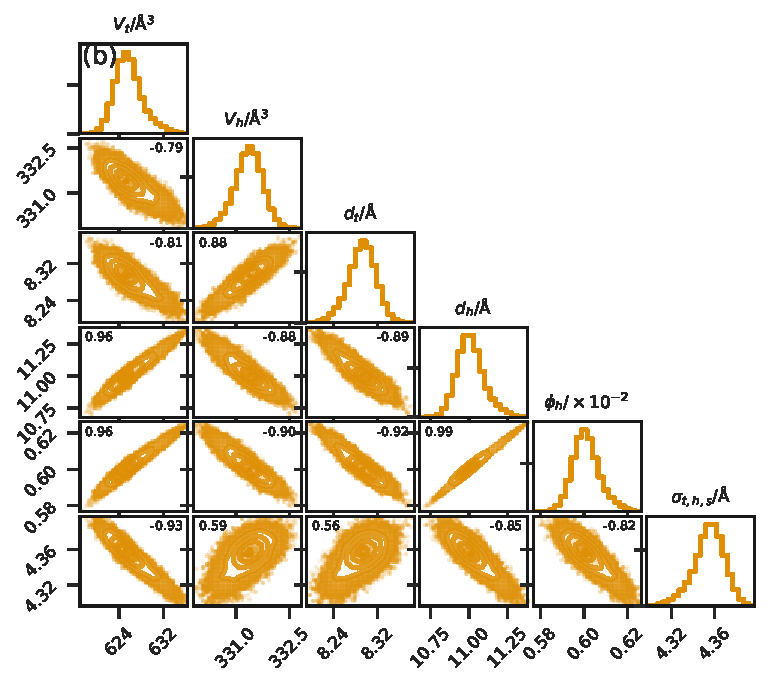
\includegraphics[width=0.49\textwidth]{reflectometry1/dlpc_xray_sp_25_pdf} \\
    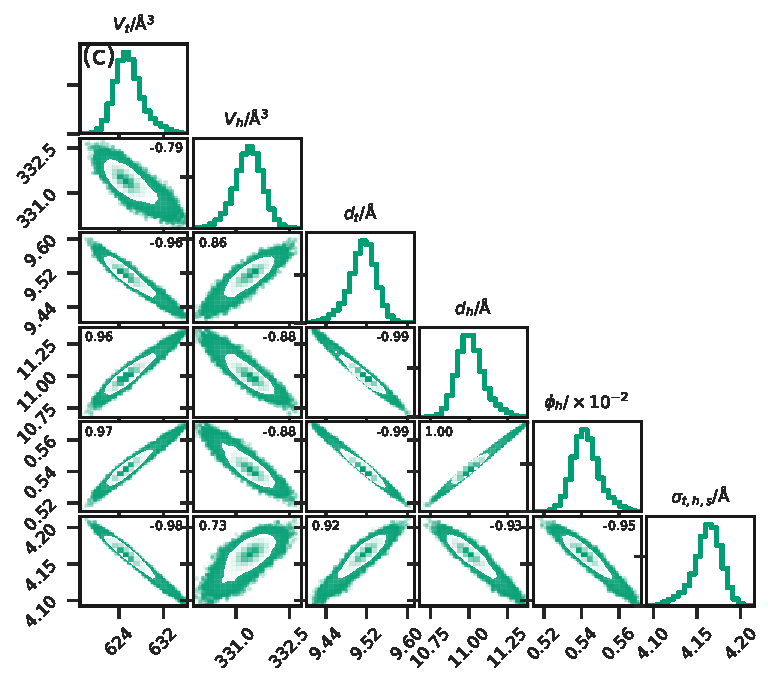
\includegraphics[width=0.49\textwidth]{reflectometry1/dlpc_xray_sp_30_pdf}
    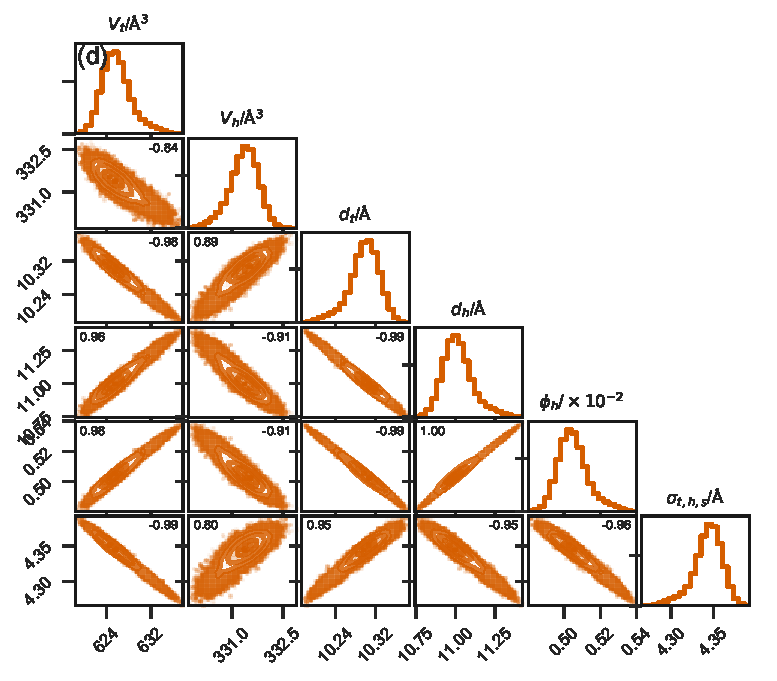
\includegraphics[width=0.49\textwidth]{reflectometry1/dlpc_xray_sp_35_pdf}
    \caption{The probability distribution functions from the chemically-consistent modelling of DLPC; (a) at \SI{20}{\milli\newton\per\meter}, (b) at \SI{25}{\milli\newton\per\meter}, (c) at \SI{30}{\milli\newton\per\meter}, (d) at \SI{35}{\milli\newton\per\meter}. The Pearson correlation coefficient for each pair of parameters is given in the top corner of each two-dimensional PDF.}
    \label{fig:dlpcpdfs}
\end{figure}
%

The sums of the magnitudes of the Pearson correlation coefficients for each PC-containing phospholipids at each surface pressures are given in Figure~\ref{fig:pear}.
From this figure, it is clear that there is a relationship between the phospholipid and the correlation present in the reflectometry model due to the skewed two-dimensional probability distribution.
This is the effect of the reduction in the phospholipid length from DPPC to DLPC, and that a corresponding decrease is not observed for the interfacial roughness.
Therefore, the boundary between phospholipid head and tail layers is less well defined.\footnote{As can be observed by investigating the SLD profiles in Figure~\ref{fig:xrrref}.}
Furthermore, the magnitude of the Pearson correlation between the head and tail thicknesses increases with increasing tail length; from $\input{output/reflectometry1/dppc_xray/dppc_p_d_t_d_h_sp30.txt}$ for DPPC, to $\input{output/reflectometry1/dmpc_xray/dmpc_p_d_t_d_h_sp30.txt}$ for DMPC, to $\input{output/reflectometry1/dlpc_xray/dlpc_p_d_t_d_h_sp30.txt}$ for DLPC, each at \SI{30}{\milli\newton\per\meter}.
Indicating that as the phospholipid tail length decreases, the negative correlation between the head and tail layers increases to the point for DLPC where the two variables are almost completely correlated and the boundary between the head and the tail is nearly nonexistent due to the magnitude of the interfacial roughness.
%
\begin{figure}
    \centering
    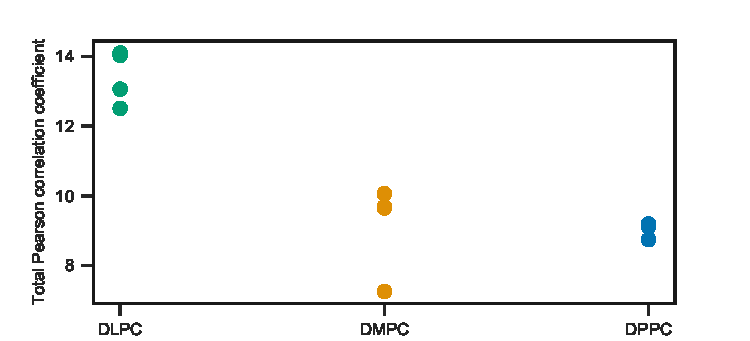
\includegraphics[width=\textwidth]{reflectometry1/pear}
    \caption{The sum of the magnitudes for each of the Pearson correlation coefficients for each of the PC-containing lipids.}
    \label{fig:pear}
\end{figure}
%

There is also a substantial positive correlation present for all of the datasets between the phospholipid head layer thickness and the volume fraction of solvent in the head layer.
This correlation can be rationalised as a result of the SLD of the solvent and the head layer\footnote{Which can be as much as \SI{78}{\percent} solvent by volume.} being similar, and therefore the boundary between the head layer and the solvent is also poorly defined.
A significant correlation such as this is unavoidable, without considering the use of many neutron contrasts for both the phospholipid and the solvent, due to the highly solvophilic nature of the head groups.
